\documentclass{article}

\usepackage{fancyhdr} % Required for custom headers
\usepackage{lastpage} % Required to determine the last page for the footer
\usepackage{extramarks} % Required for headers and footers
\usepackage[usenames,dvipsnames]{color} % Required for custom colors
\usepackage{graphicx} % Required to insert images
\usepackage{listings} % Required for insertion of code
\usepackage{courier} % Required for the courier font
\usepackage{lipsum} % Used for inserting dummy 'Lorem ipsum' text into the template
\usepackage{amsmath}
\usepackage{amssymb}
\usepackage{mathtools, xparse}
\usepackage{booktabs}
\usepackage{bigstrut}
\usepackage{float}
\usepackage{hyperref}
\usepackage{color}
\usepackage{algorithm}
\usepackage{caption}
\captionsetup{skip=0pt}
\usepackage{algpseudocode}
\usepackage{multirow}
\usepackage{subfigure}
\usepackage{longtable}
\usepackage{supertabular}
\usepackage{biblatex}

\renewcommand*{\Rnfont}{\scshape}

\DeclarePairedDelimiter{\norm}{\lVert}{\rVert}
\DeclarePairedDelimiter\abs{\lvert}{\rvert}%

\hypersetup{
    colorlinks   = true,    % Colours links instead of ugly boxes
    urlcolor     = red,    % Colour for external hyperlinks
    linkcolor    = red,    % Colour of internal links
    citecolor    = red      % Colour of citations
}
% Margins
\topmargin=-0.45in
\evensidemargin=0in
\oddsidemargin=0in
\textwidth=6.5in
\textheight=9.0in
\headsep=0.25in

\linespread{1.1} % Line spacing

% Set up the header and footer
\pagestyle{fancy}
\lhead{\hmwkAuthorName} % Top left header
\rhead{\hmwkClass\ : \hmwkID} % Top center head
%\rhead{\firstxmark} % Top right header
\lfoot{\lastxmark} % Bottom left footer
\cfoot{} % Bottom center footer
\rfoot{Page\ \thepage\ of\ \protect\pageref*{LastPage}} % Bottom right footer
\renewcommand\headrulewidth{0.4pt} % Size of the header rule
\renewcommand\footrulewidth{0.4pt} % Size of the footer rule
\renewcommand{\subsectionmark}[1]{\markboth{#1}{}}
\setlength\parindent{0pt} % Removes all indentation from paragraphs

%----------------------------------------------------------------------------------------
%	CODE INCLUSION CONFIGURATION
%----------------------------------------------------------------------------------------

\definecolor{MyDarkGreen}{rgb}{0.0,0.4,0.0} % This is the color used for comments
\lstloadlanguages{Perl} % Load Perl syntax for listings, for a list of other languages supported see: ftp://ftp.tex.ac.uk/tex-archive/macros/latex/contrib/listings/listings.pdf
\lstset{language=Perl, % Use Perl in this example
    frame=single, % Single frame around code
    basicstyle=\small\ttfamily, % Use small true type font
    keywordstyle=[1]\color{Blue}\bf, % Perl functions bold and blue
    keywordstyle=[2]\color{Purple}, % Perl function arguments purple
    keywordstyle=[3]\color{Blue}\underbar, % Custom functions underlined and blue
    identifierstyle=, % Nothing special about identifiers                                         
    commentstyle=\usefont{T1}{pcr}{m}{sl}\color{MyDarkGreen}\small, % Comments small dark green courier font
    stringstyle=\color{Purple}, % Strings are purple
    showstringspaces=false, % Don't put marks in string spaces
    tabsize=5, % 5 spaces per tab
    %
    % Put standard Perl functions not included in the default language here
    morekeywords={rand},
    %
    % Put Perl function parameters here
    morekeywords=[2]{on, off, interp},
    %
    % Put user defined functions here
    morekeywords=[3]{test},
    %
    morecomment=[l][\color{Blue}]{...}, % Line continuation (...) like blue comment
    numbers=left, % Line numbers on left
    firstnumber=1, % Line numbers start with line 1
    numberstyle=\tiny\color{Blue}, % Line numbers are blue and small
    stepnumber=5 % Line numbers go in steps of 5
}

% Creates a new command to include a perl script, the first parameter is the filename of the script (without .pl), the second parameter is the caption
\newcommand{\perlscript}[2]{
    \begin{itemize}
        \item[]\lstinputlisting[caption=#2,label=#1]{#1.py}
    \end{itemize}
}
\newcommand{\cppscript}[1]{
    \begin{itemize}
        \item[]\lstinputlisting[]{#1}
    \end{itemize}
}

%----------------------------------------------------------------------------------------
%	DOCUMENT STRUCTURE COMMANDS
%	Skip this unless you know what you're doing
%----------------------------------------------------------------------------------------

% Header and footer for when a page split occurs within a problem environment
\newcommand{\enterProblemHeader}[1]{
    \nobreak\extramarks{#1}{#1 continued on next page\ldots}\nobreak
    \nobreak\extramarks{#1 (continued)}{#1 continued on next page\ldots}\nobreak
}

% Header and footer for when a page split occurs between problem environments
\newcommand{\exitProblemHeader}[1]{
    \nobreak\extramarks{#1 (continued)}{#1 continued on next page\ldots}\nobreak
    \nobreak\extramarks{#1}{}\nobreak
}

%\setcounter{secnumdepth}{0} % Removes default section numbers
\newcounter{homeworkProblemCounter} % Creates a counter to keep track of the number of problems

\newcommand{\homeworkProblemName}{}
\newenvironment{homeworkProblem}[1][Problem \arabic{homeworkProblemCounter}]{ % Makes a new environment called homeworkProblem which takes 1 argument (custom name) but the default is "Problem #"
    \stepcounter{homeworkProblemCounter} % Increase counter for number of problems
    \renewcommand{\homeworkProblemName}{#1} % Assign \homeworkProblemName the name of the problem
    \section{\homeworkProblemName} % Make a section in the document with the custom problem count
    \enterProblemHeader{\homeworkProblemName} % Header and footer within the environment
    }{
    \exitProblemHeader{\homeworkProblemName} % Header and footer after the environment
}

\newcommand{\problemAnswer}[1]{ % Defines the problem answer command with the content as the only argument
\noindent\framebox[\columnwidth][c]{\begin{minipage}{0.98\columnwidth}#1\end{minipage}} % Makes the box around the problem answer and puts the content inside
}

\newcommand{\homeworkSectionName}{}
\newenvironment{homeworkSection}[1]{ % New environment for sections within homework problems, takes 1 argument - the name of the section
    \renewcommand{\homeworkSectionName}{#1} % Assign \homeworkSectionName to the name of the section from the environment argument
    \subsection{\homeworkSectionName} % Make a subsection with the custom name of the subsection
    \enterProblemHeader{\homeworkProblemName\ [\homeworkSectionName]} % Header and footer within the environment
    }{
    \enterProblemHeader{\homeworkProblemName} % Header and footer after the environment
}

%----------------------------------------------------------------------------------------
%	NAME AND CLASS SECTION
%----------------------------------------------------------------------------------------

\newcommand{\hmwkID}{hw04-1} % Assignment title
\newcommand{\hmwkTitle}{Single Element Synthetic Aperture Focusing}
\newcommand{\hmwkDueDate}{Thursday,\ Nov\ 16,\ 2017} % Due date
\newcommand{\hmwkClass}{Principles of Biomedical Ultrasound and Photoacoustics} % Course/class
\newcommand{\hmwkClassTime}{10:30am} % Class/lecture time
\newcommand{\hmwkClassInstructor}{Jones} % Teacher/lecturer
\newcommand{\hmwkAuthorName}{106061531 Fu-En Wang} % Your name

%----------------------------------------------------------------------------------------
%	TITLE PAGE
%----------------------------------------------------------------------------------------

\title{
    \vspace{2in}
    \textmd{\textbf{\hmwkClass}}\\
    \textmd{\textbf{\hmwkID: \hmwkTitle}} \\
    \normalsize\vspace{0.1in}\small{Due\ on\ \hmwkDueDate}\\
    \vspace{3in}
}

\author{\textbf{\hmwkAuthorName}}
\date{} % Insert date here if you want it to appear below your name

%----------------------------------------------------------------------------------------

\begin{document}
\maketitle
\newpage

\renewcommand\thesubsection{\thesection.\alph{subsection}}

\section{Introduction}
In this homework, we will simulate phased array system beam forming.
\begin{figure}[H]
    \centering
    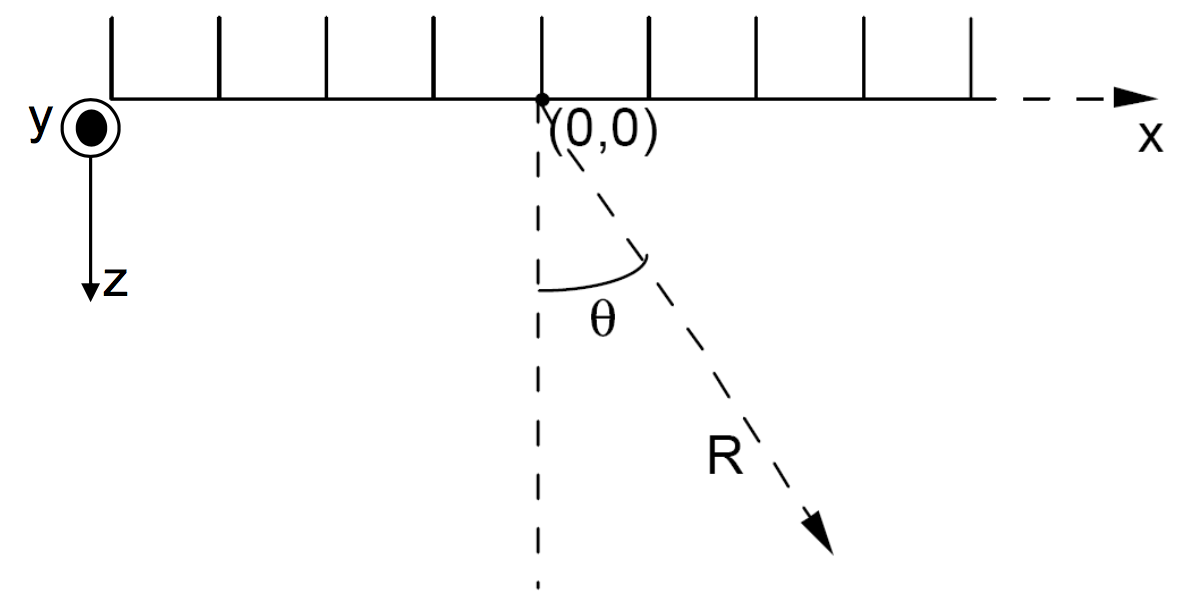
\includegraphics[width = 0.6\textwidth]{src/phase-system.png}
    \caption{Phase array system}
\end{figure}

To create the channel data, we can follow the steps below.
\begin{enumerate}
    \item The transmitter (i.e., each array element) is a perfect point source
    \item The receiver (i.e., each array element) is a perfect point receiver
    \item There is no attenuation. That is, the received signal does not need to be gain compensated.
    \item The sound speed is 1.5 mm/us or 1500 m/s
    \item The complete channel data are collected with consecutive single element transmitting and receiving.
    \item The position of the 3 point targets in (x,y,z): (-5, 0, 10), (0, 0, 20), (15,0,30) in mm.
    \item The initial sampling rate (i.e., fs) is set to 64*fc to emulate “analog” channel data
    \item Perform decimation on emulated “analog” channel data so that the resultant sampling rate (i.e., fs) is 4*fc on 
          “sampled” channel data
    \item Make wavefield plots of the “analog” and “sampled” data (i.e., image of channel data). The gray scale is setup so that zero 
          pressure is midgray, positive pressure is white, and negative pressure is black.
\end{enumerate}


\section{Problems}
Implement RF and baseband dynamic receive beamformer to make a 120-degree sector scan image from the sampled channel data.

\subsection{Define beam spacing and the number of total beams}
The beam space is uniformly divided in sine space.
$$
    \Delta \sin\theta = \frac{\lambda}{2D} = 0.0156
$$
in mm. The number of beams is
$$
    \frac{\sqrt{3}}{\Delta \sin\theta} = 111
$$

\subsection{RF and baseband beamforming}
Now we show beamforming of RF and Baseband as shown in Figure [\ref{fig:RF-b-9} \ref{fig:Base-b-6}].
\begin{figure}[H]
    \centering
    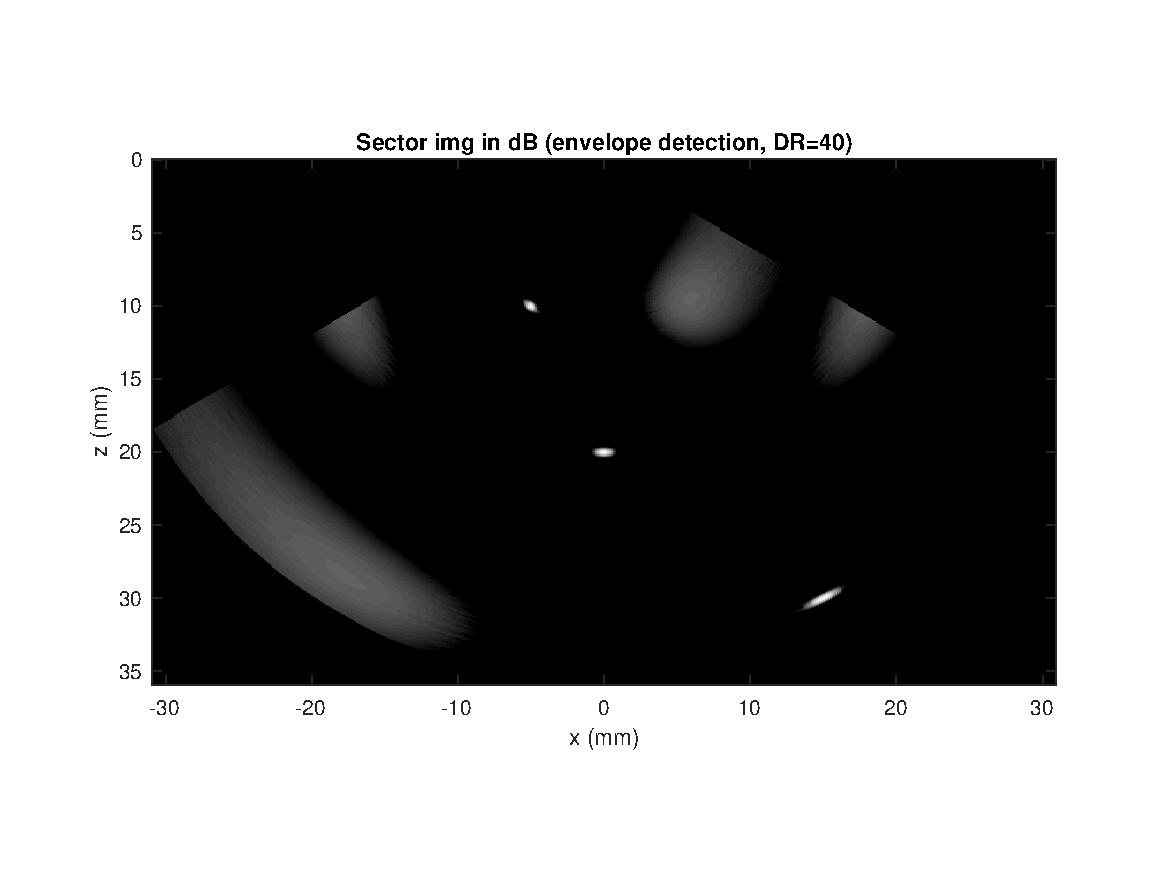
\includegraphics[width=0.5\textwidth]{src/RF/b-9.pdf}
    \caption{Sector image (RF)}
    \label{fig:RF-b-9}
\end{figure}
\begin{figure}[H]
    \centering
    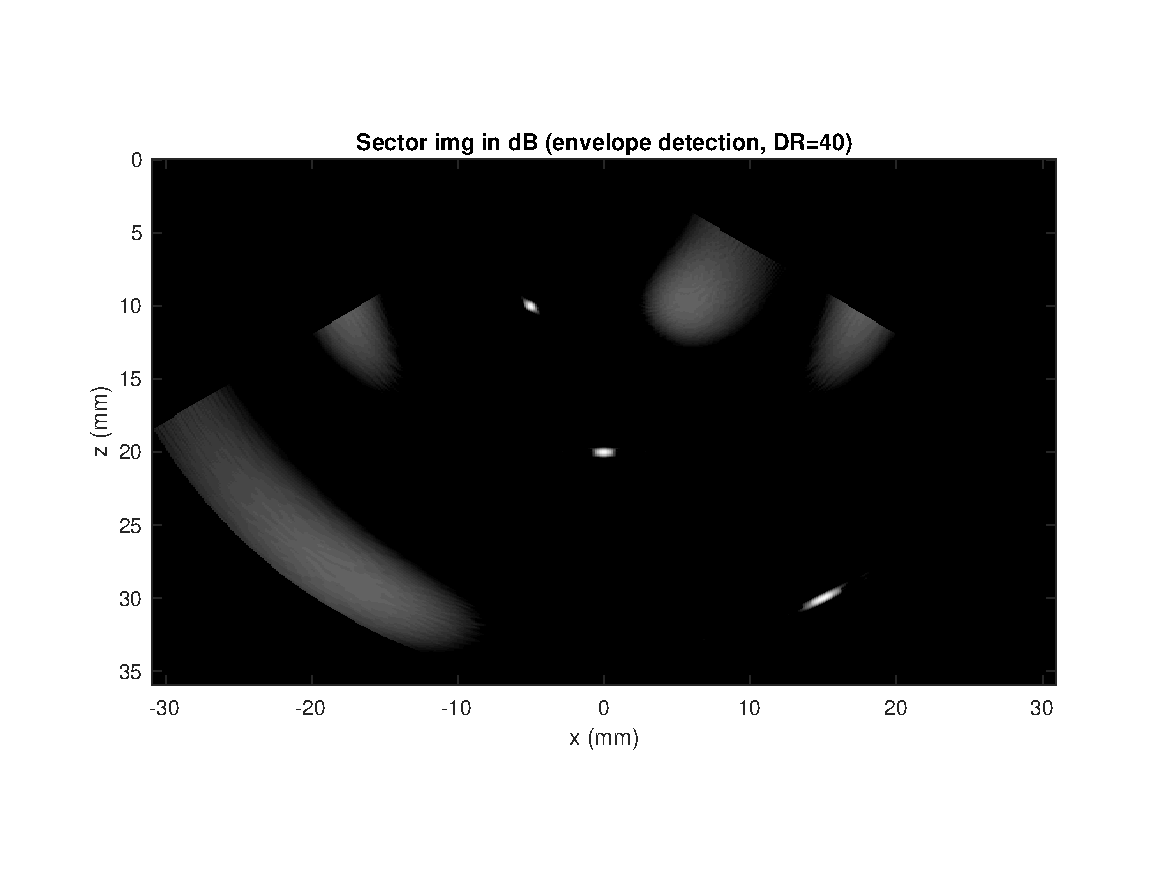
\includegraphics[width=0.5\textwidth]{src/Base/b-6.pdf}
    \caption{Sector image (Baseband)}
    \label{fig:Base-b-6}
\end{figure}

Figure \ref{fig:RF-fft-origin} show the original spectrum of center scanline for RF beamforming.
\begin{figure}[H]
    \centering
    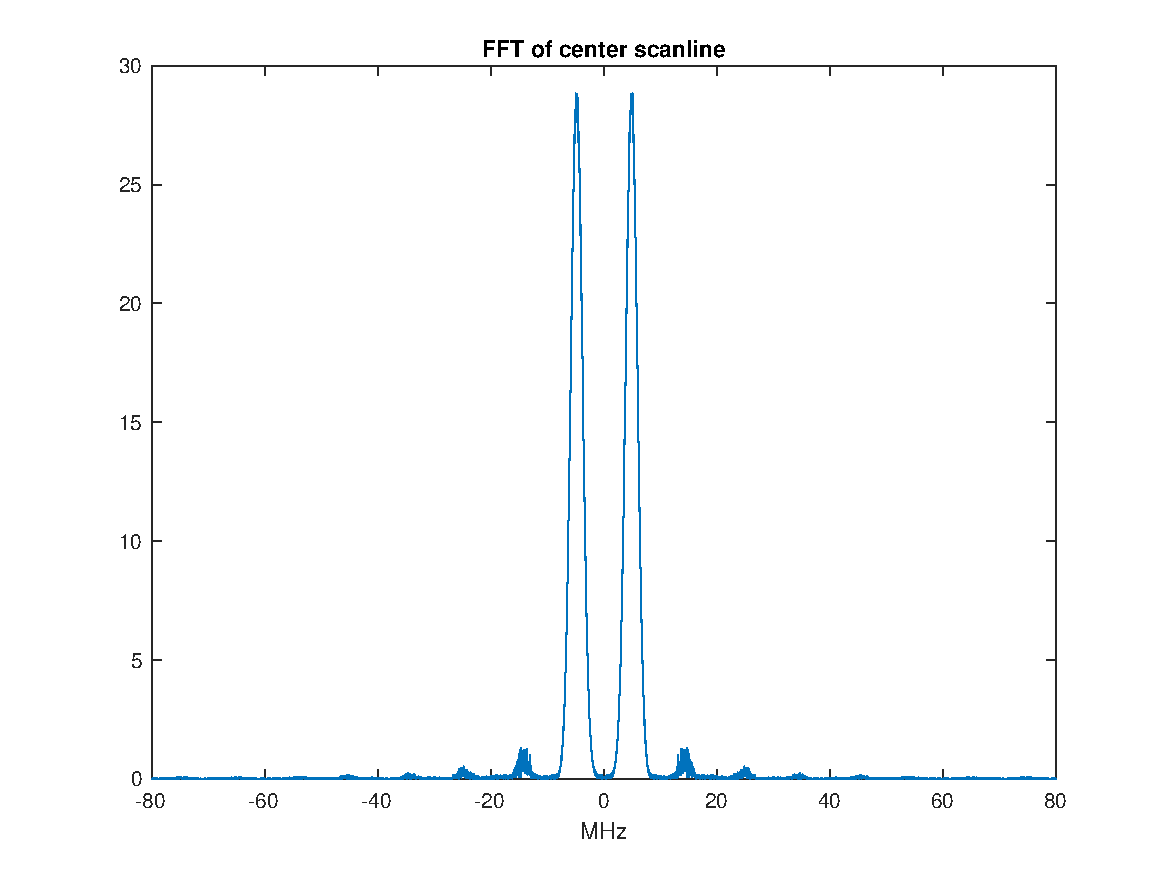
\includegraphics[width=0.6\textwidth]{src/RF/b-4.pdf}
    \caption{FFT (origin)}
    \label{fig:RF-fft-origin}
\end{figure}
Now we apply demodulation with the following formula
$$
    BBbeam = BBbeam * \exp^{-2 \pi * fc * t * j}
$$
And the spectrum will shift -fc as shown in Figure \ref{fig:RF-fft-shift}
\begin{figure}[H]
    \centering
    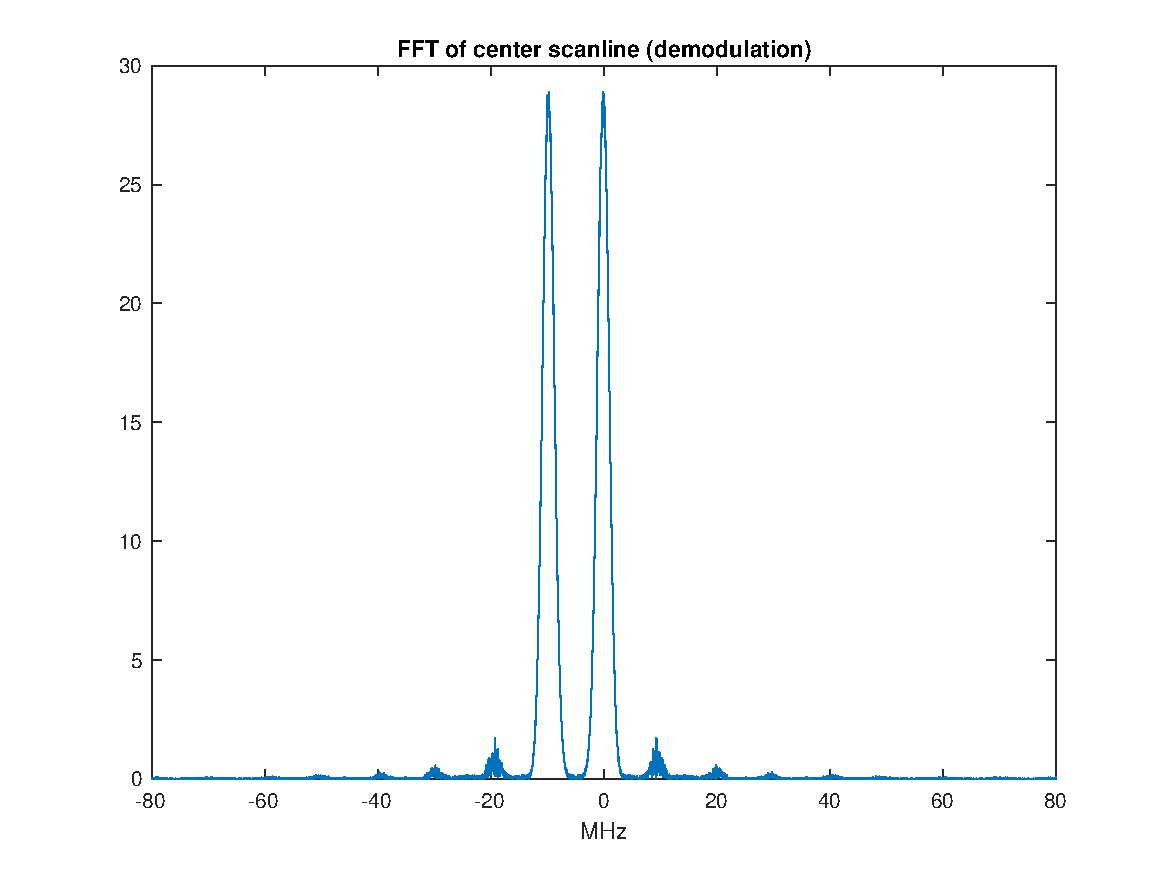
\includegraphics[width=0.6\textwidth]{src/RF/b-5.pdf}
    \caption{FFT (demodulation)}
    \label{fig:RF-fft-shift}
\end{figure}
Now we apply a low pass filter with cutoff frquency fc (Figure \ref{fig:RF-LPF}) to preserve the main lobe only 
(Figure \ref{fig:RF-fft-shift-LPF})
\begin{figure}[H]
    \centering
    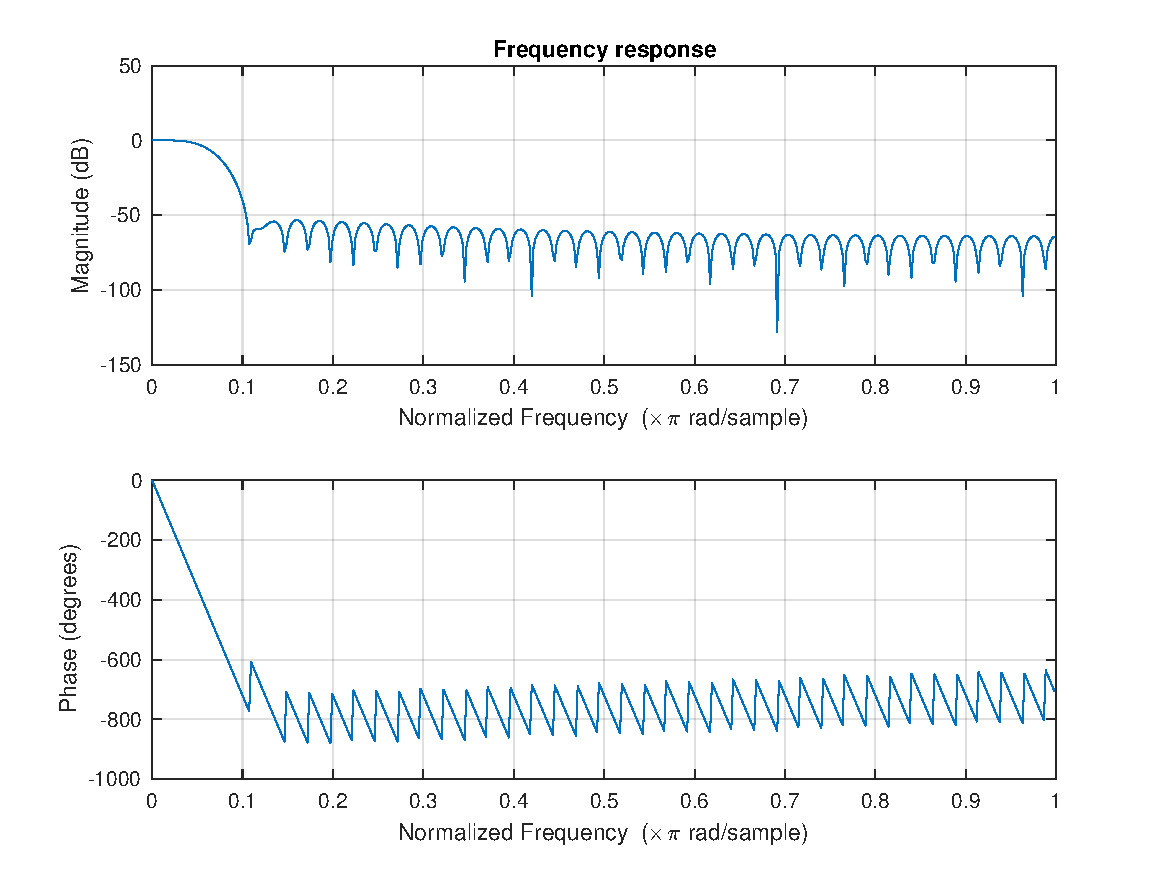
\includegraphics[width=0.6\textwidth]{src/RF/b-6.pdf}
    \caption{LPF frequency response}
    \label{fig:RF-LPF}
\end{figure}
\begin{figure}[H]
    \centering
    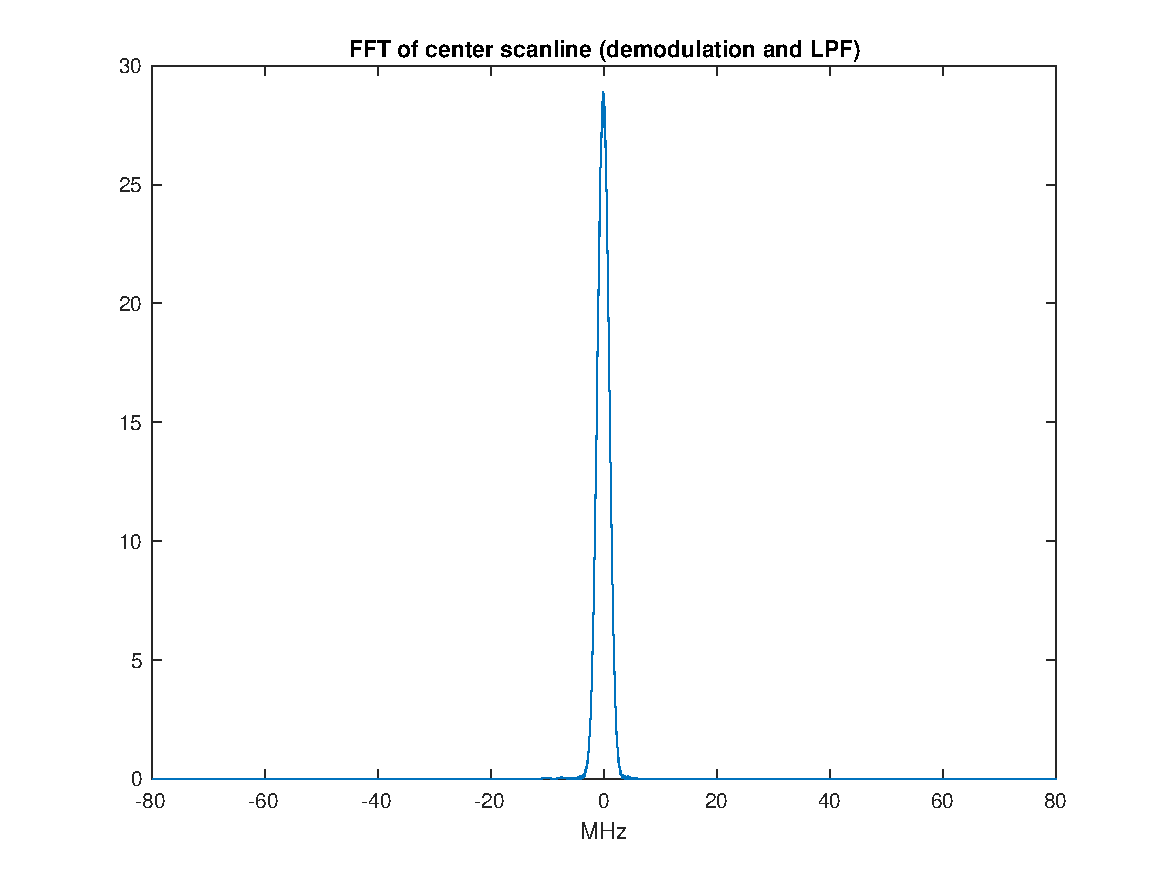
\includegraphics[width=0.6\textwidth]{src/RF/b-7.pdf}
    \caption{FFT (demodulation and LPF)}
    \label{fig:RF-fft-shift-LPF}
\end{figure}
Now we finish all steps of baseband demodulation.

\subsection{Create baseband data (Matlab: ones())}
When the \textbf{w} in source code is assigned by \textbf{ones}, the beam buffer of RF and Baseband after beamforming is shown in
Figure \ref{fig:RF-ones} and \ref{fig:Base-ones}, respectively.
\begin{figure}[H]
    \centering
    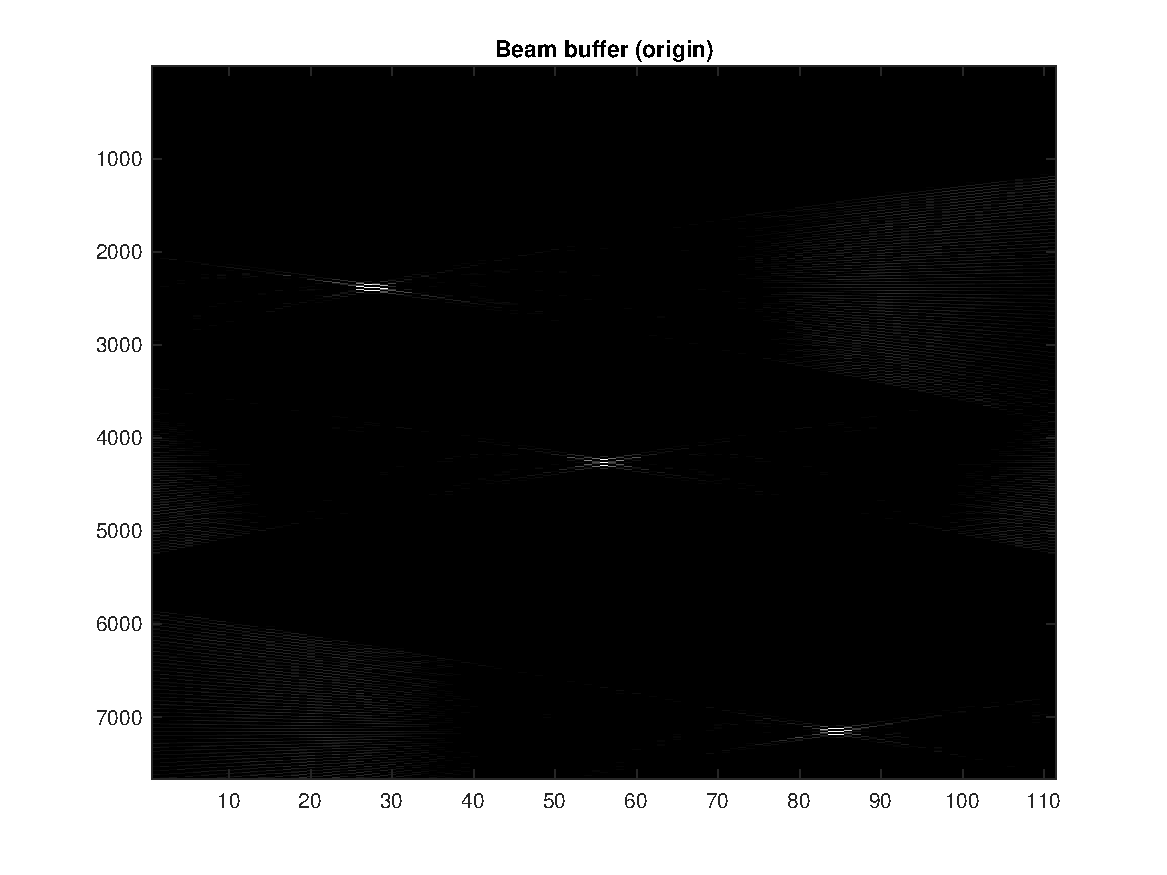
\includegraphics[width=0.6\textwidth]{src/RF/b-3-ones.pdf}
    \caption{Beam buffer of RF(ones)}
    \label{fig:RF-ones}
\end{figure}
\begin{figure}[H]
    \centering
    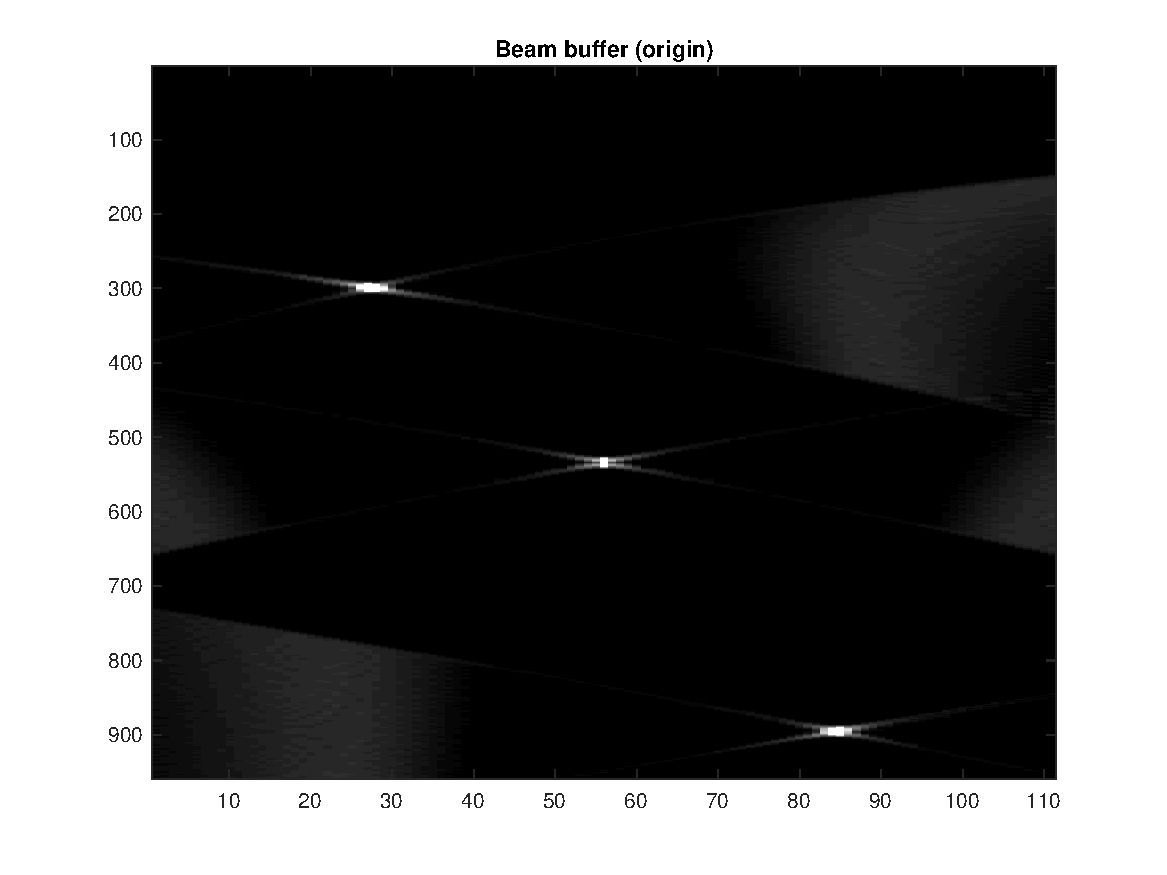
\includegraphics[width=0.6\textwidth]{src/Base/b-4-ones.pdf}
    \caption{Beam buffer of Baseband(ones)}
    \label{fig:Base-ones}
\end{figure}


\subsection{Create baseband data (Matlab: hanning())}
When the \textbf{w} in source code is assigned by \textbf{hanning}, the beam buffer of RF and Baseband after beamforming is shown in
Figure \ref{fig:RF-hanning} and \ref{fig:Base-hanning}, respectively.
\begin{figure}[H]
    \centering
    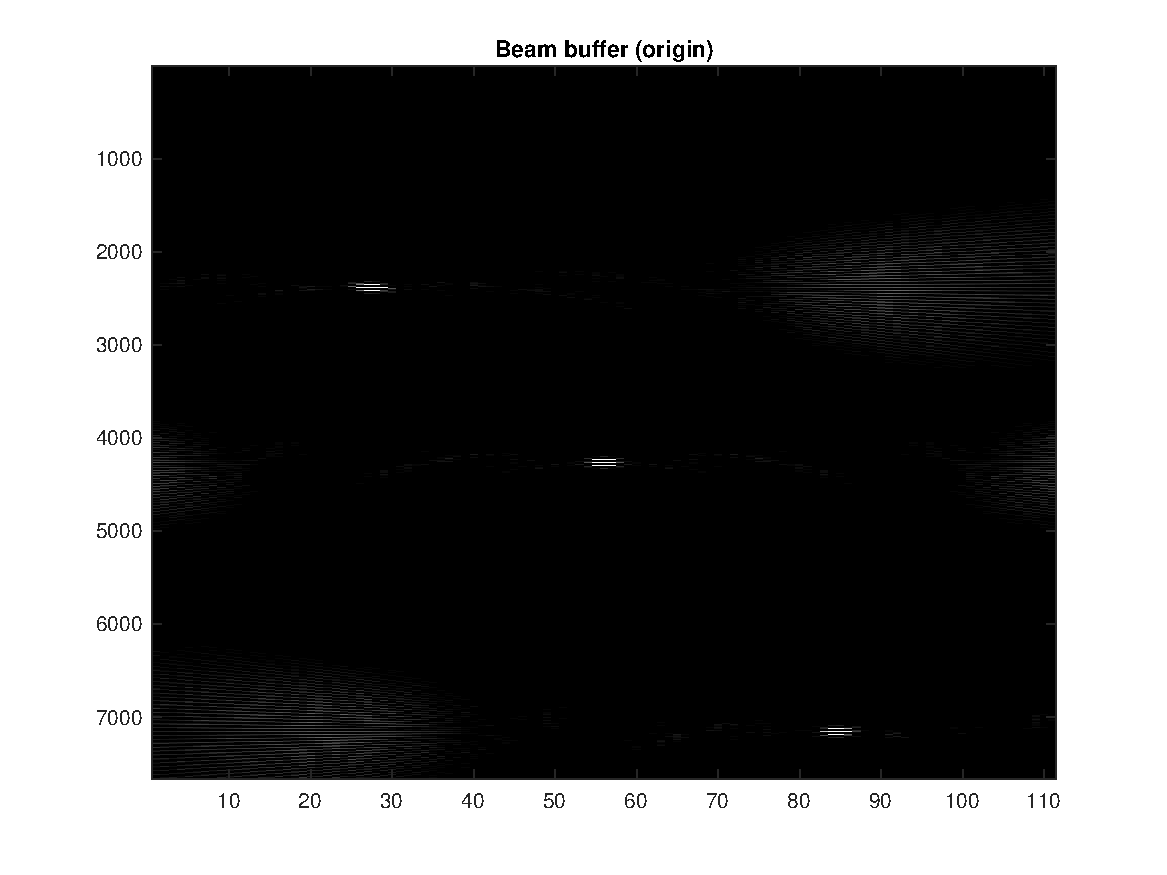
\includegraphics[width=0.6\textwidth]{src/RF/b-3-hanning.pdf}
    \caption{Beam buffer of RF (hanning)}
    \label{fig:RF-hanning}
\end{figure}
\begin{figure}[H]
    \centering
    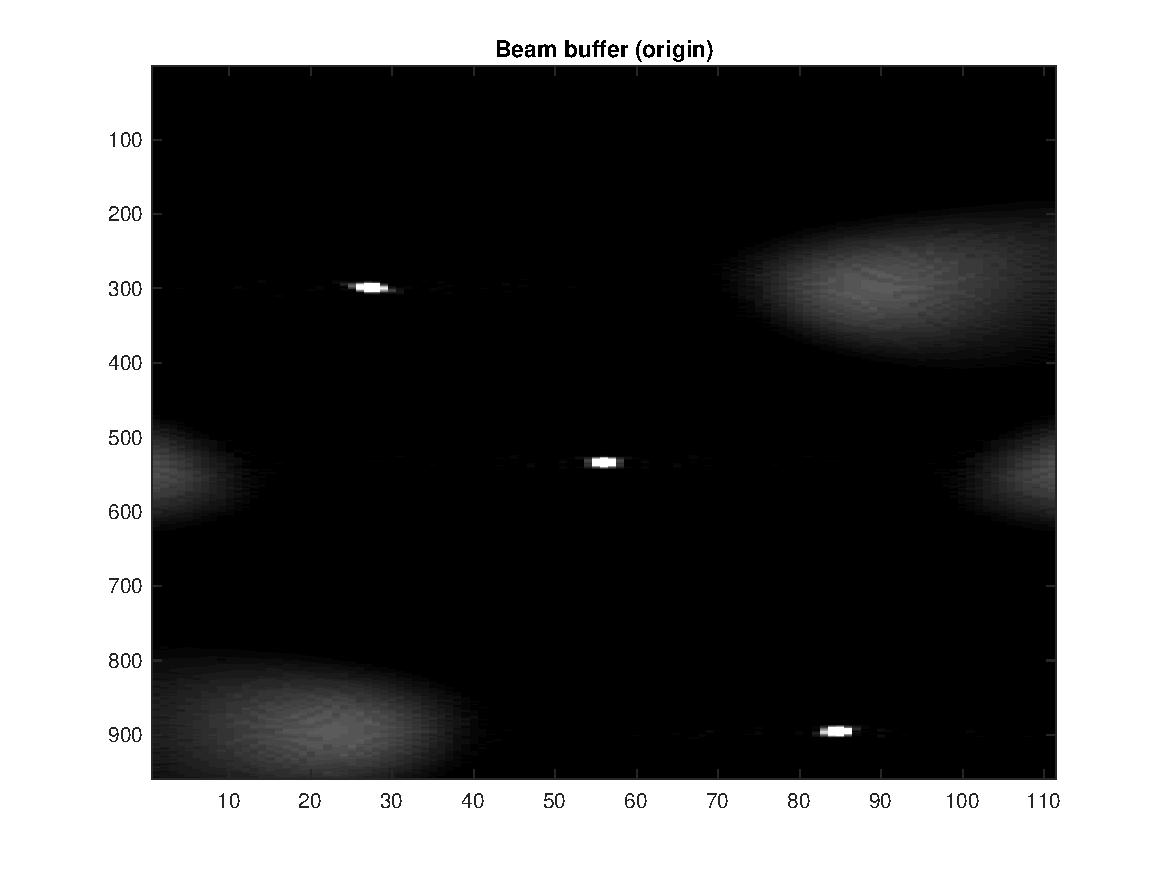
\includegraphics[width=0.6\textwidth]{src/Base/b-4-hanning.pdf}
    \caption{Beam buffer of Baseband (hanning)}
    \label{fig:Base-hanning}
\end{figure}


\subsection{Create baseband data ($\Delta \sin \theta = \lambda / D$)}
Figure \ref{fig:RF-ones-1D} shows the result
\begin{figure}[H]
    \centering
    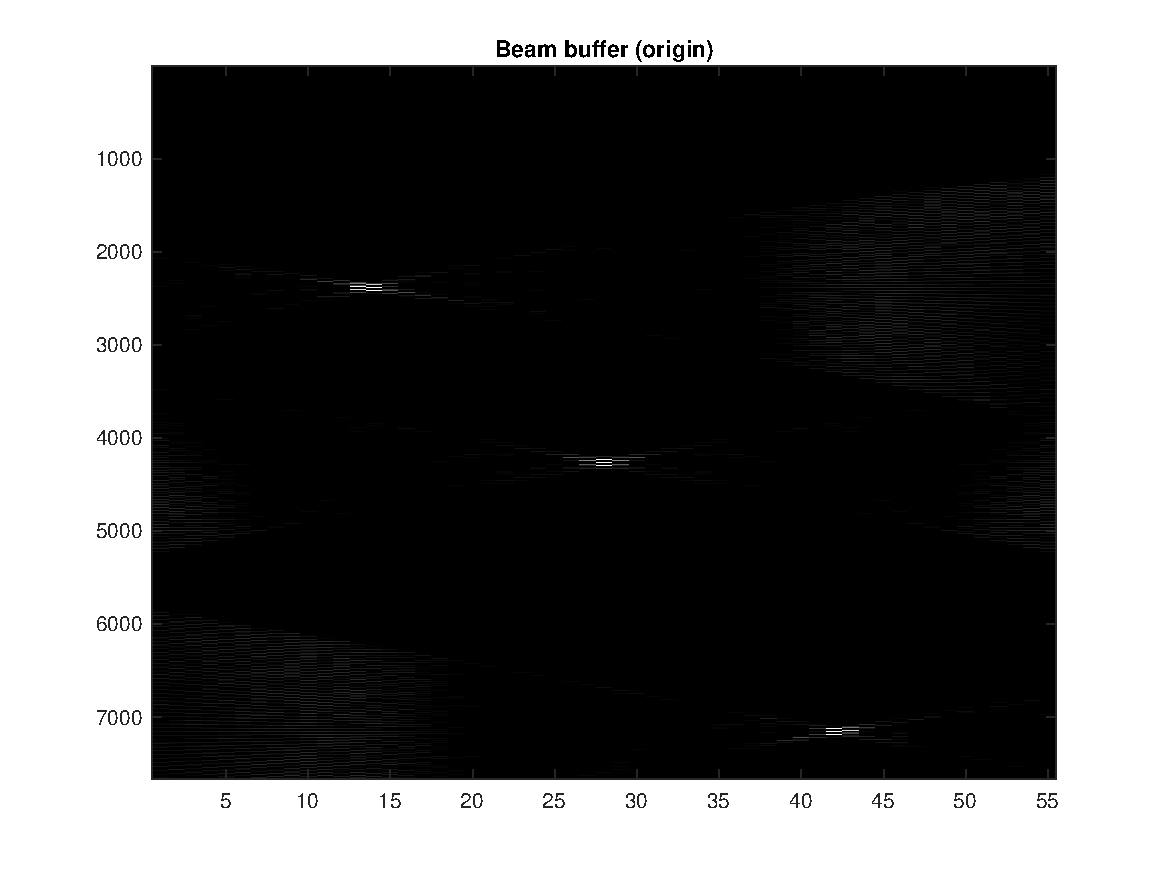
\includegraphics[width=0.6\textwidth]{src/RF/b-3-ones-1D.pdf}
    \caption{Beam buffer of RF ($\Delta \sin \theta = \lambda / D$)}
    \label{fig:RF-ones-1D}
\end{figure}

\subsection{Create baseband data}
Create baseband data for the R-sin beam buffer by computing the coherent sum across every other element (required for either RF or 
baseband beamforming only).
\begin{figure}[H]
    \centering
    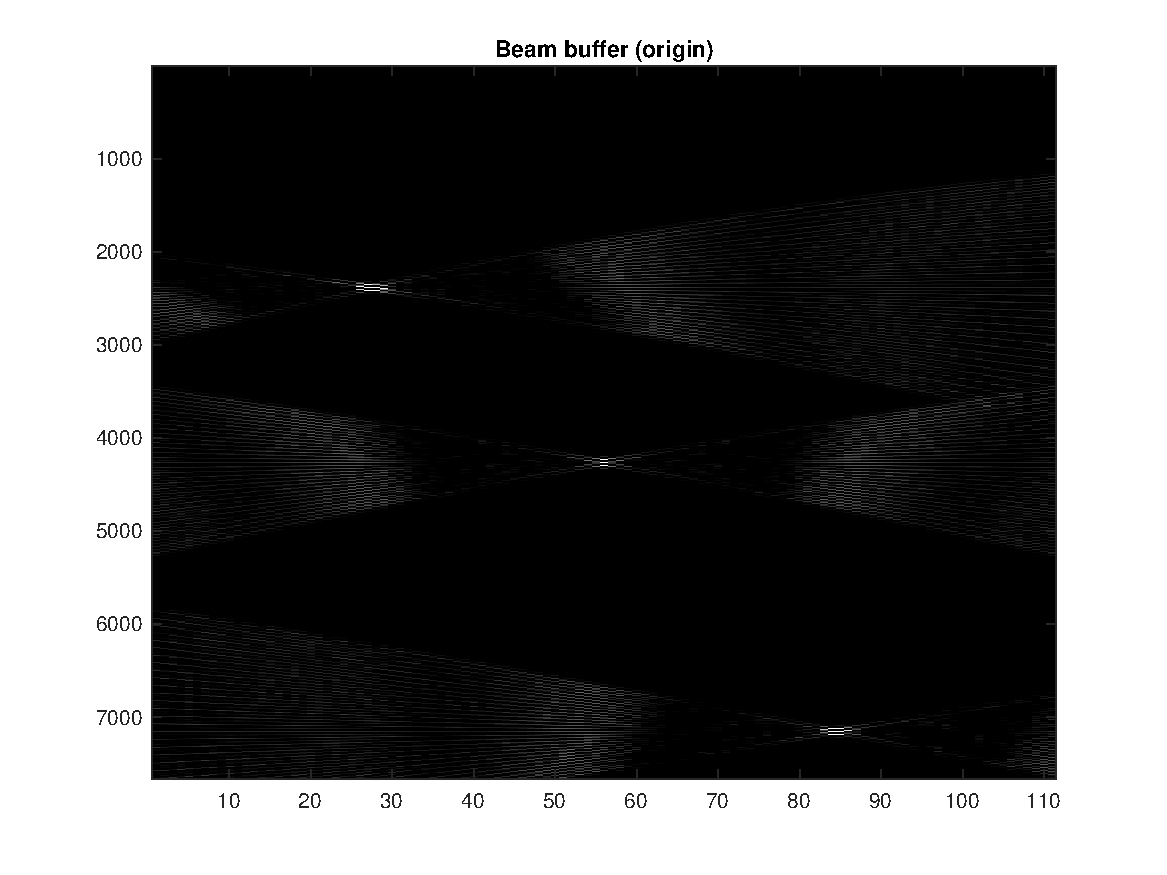
\includegraphics[width=0.6\textwidth]{src/RF/b-3-ones-everyother.pdf}
    \caption{Beam buffer of RF (every other element)}
    \label{fig:RF-ones-everyones}
\end{figure}


\subsection{Display beam buffer with 40 dB dynamic range}
Figure \ref{fig:RF-b-40db} and \ref{fig:Base-b-40db} show the result of RF and Baseband in (c), respectively.
\begin{figure}[H]
    \centering
    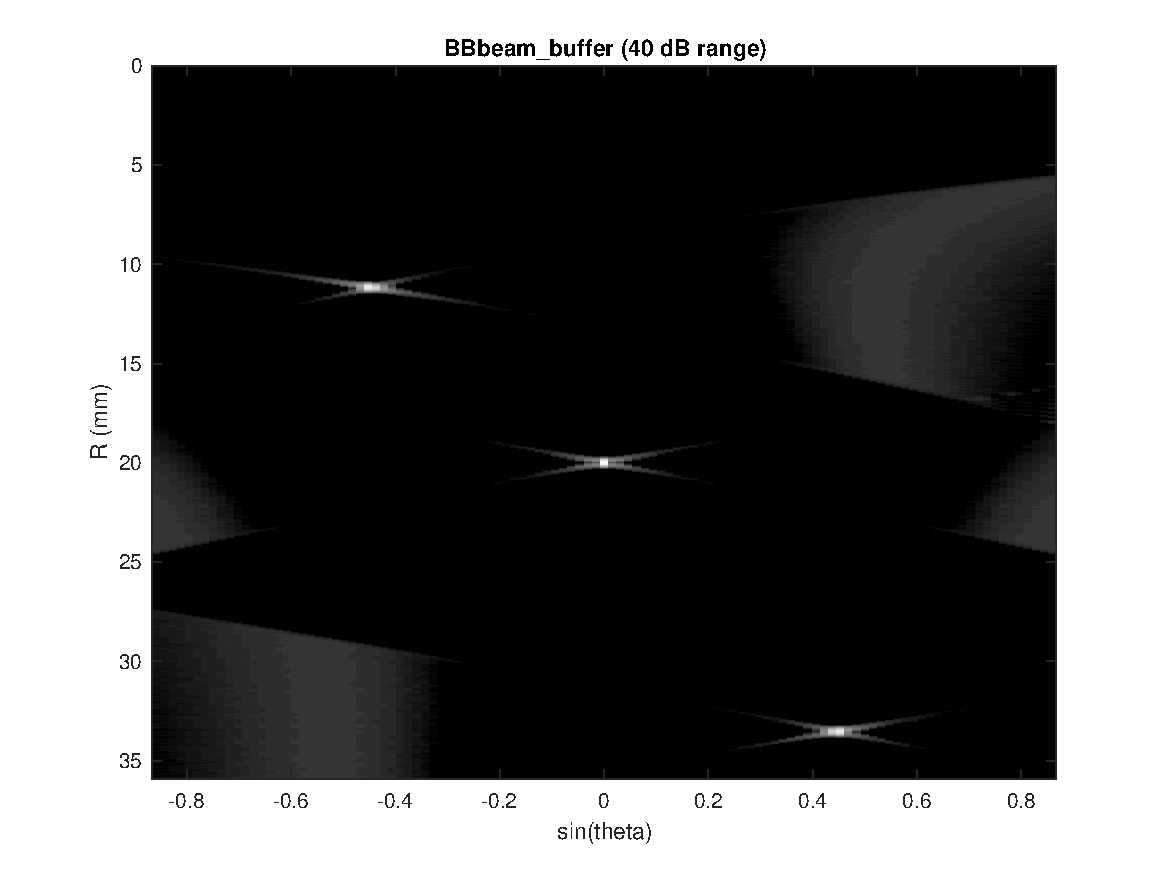
\includegraphics[width=0.6\textwidth]{src/RF/b-8.pdf}
    \caption{(c) Beam buffer of RF (40 dB dynamic range)}
    \label{fig:RF-b-40db}
\end{figure}
\begin{figure}[H]
    \centering
    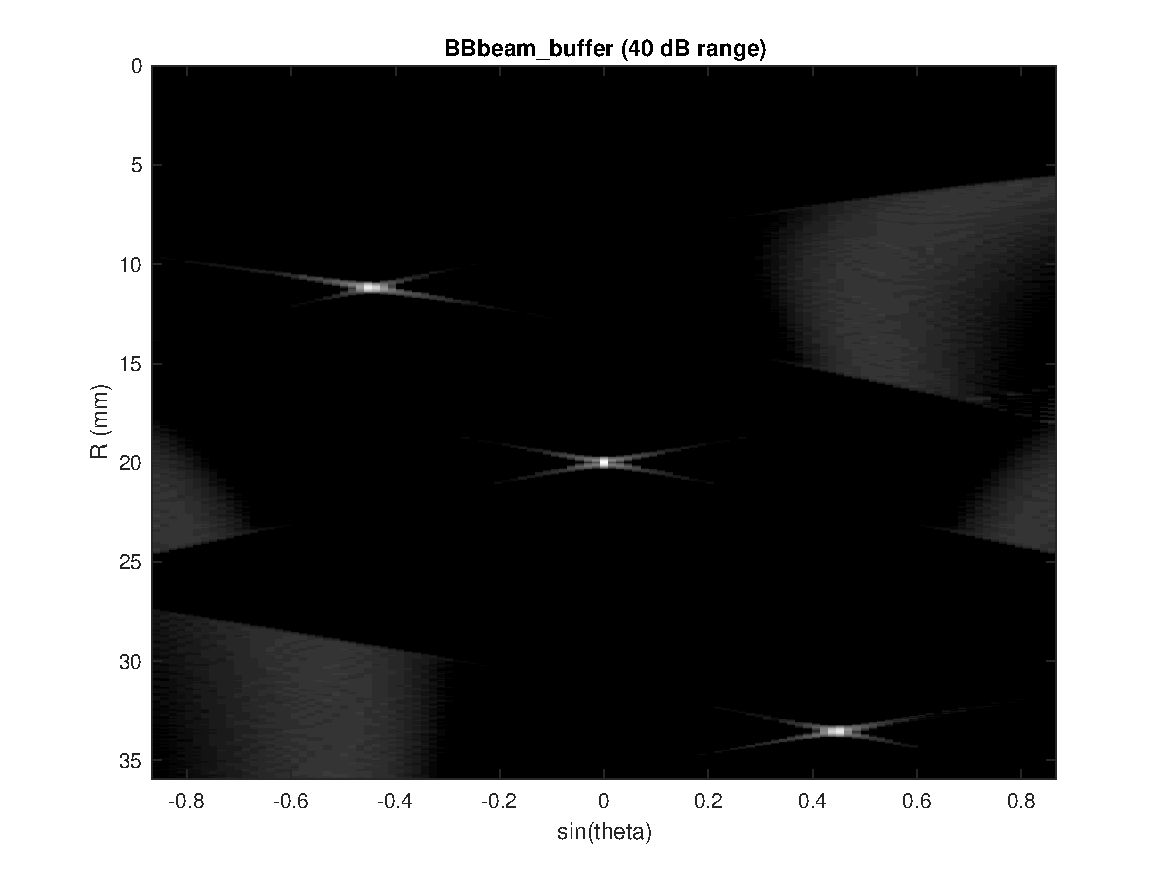
\includegraphics[width=0.6\textwidth]{src/Base/b-5.pdf}
    \caption{(c) Beam buffer of Baseband (40 dB dynamic range)}
    \label{fig:Base-b-40db}
\end{figure}
In Figure \ref{fig:RF-b-40db} and \ref{fig:Base-b-40db}, the result of RF is a little smoother than that of baseband, but I think
their results are such similar that I cannot tell difference from them.

Figure \ref{fig:RF-hanning-40db} show the 40dB result for (d).
\begin{figure}[H]
    \centering
    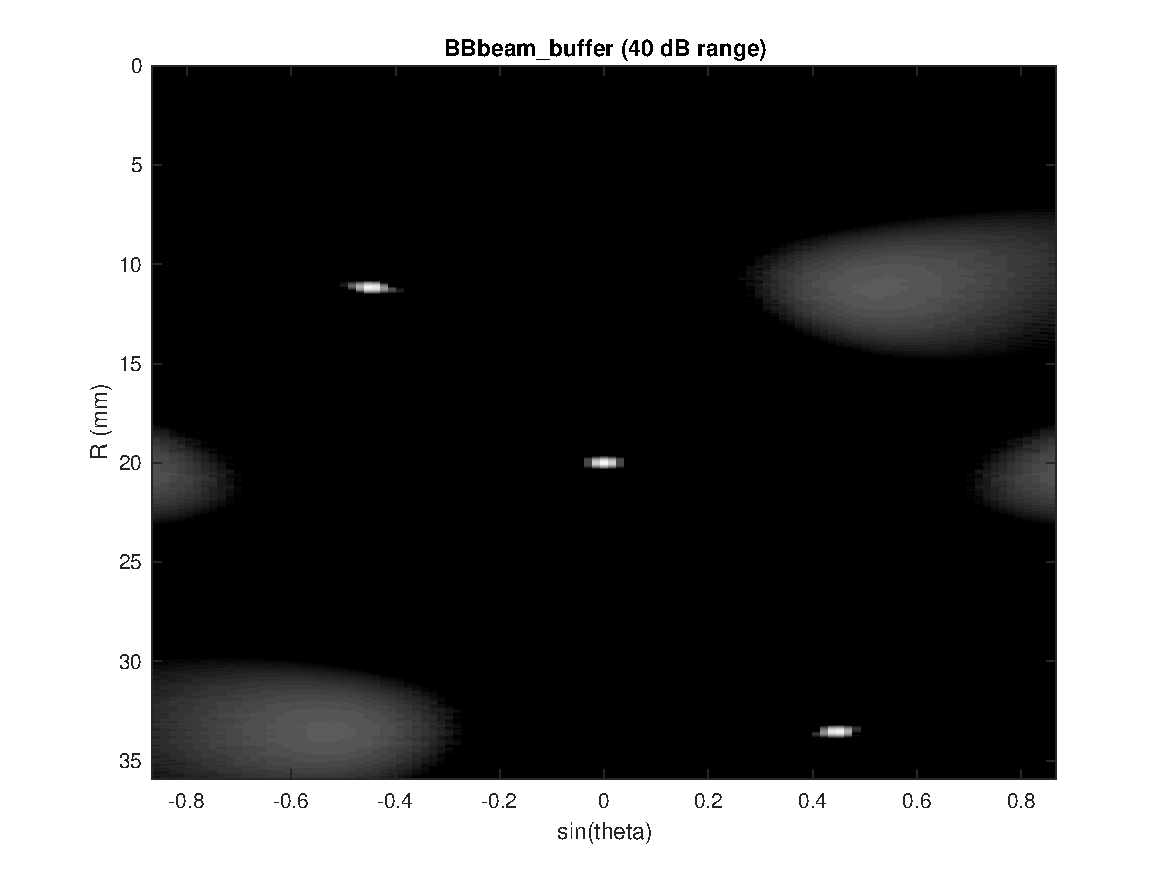
\includegraphics[width=0.6\textwidth]{src/RF/b-8-hanning.pdf}
    \caption{(d) Beam buffer of RF (40 dB dynamic range)}
    \label{fig:RF-hanning-40db}
\end{figure}
Compared with Figure \ref{fig:RF-b-40db}, the focus points in Figure \ref{fig:RF-hanning-40db} are just more like a \textbf{point}.
This is because the main lobe width of hanning window is wider than a rectangular window (ones()), and this can be seen as a smooth
operation. So the result in figure \ref{fig:RF-hanning-40db} seems better.

Figure \ref{fig:RF-2pitch-40db} show the 40dB result for (e).
\begin{figure}[H]
    \centering
    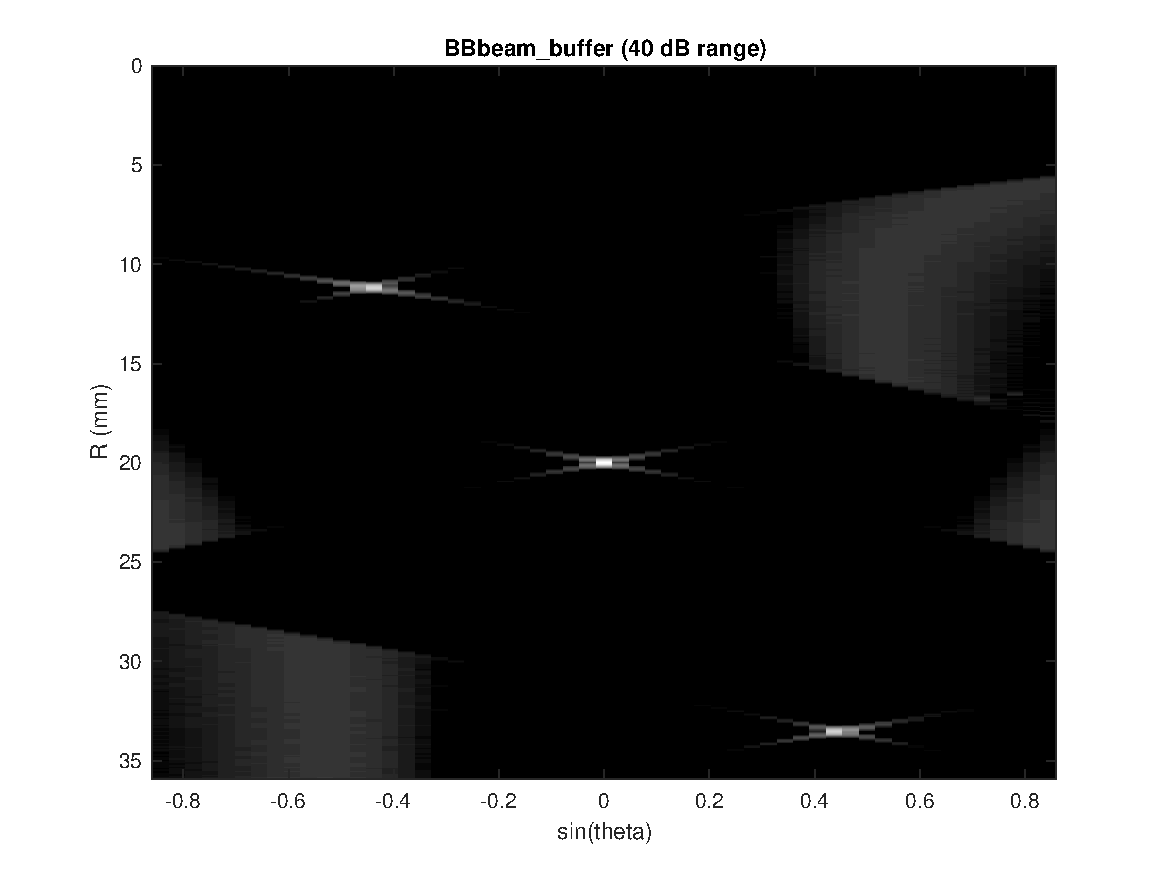
\includegraphics[width=0.6\textwidth]{src/RF/b-8-2pitch.pdf}
    \caption{(e) Beam buffer of RF (40 dB dynamic range)}
    \label{fig:RF-2pitch-40db}
\end{figure}
Because we increase the pitch (i.e distance between each $\sin \theta$ line increases), the total number of sample line decreases.
As a result, we can see a poorer resolution in Figure \ref{fig:RF-2pitch-40db} than in Figure \ref{fig:RF-b-40db}.

Figure \ref{fig:RF-everyones-40db} show the 40dB result for (f).
\begin{figure}[H]
    \centering
    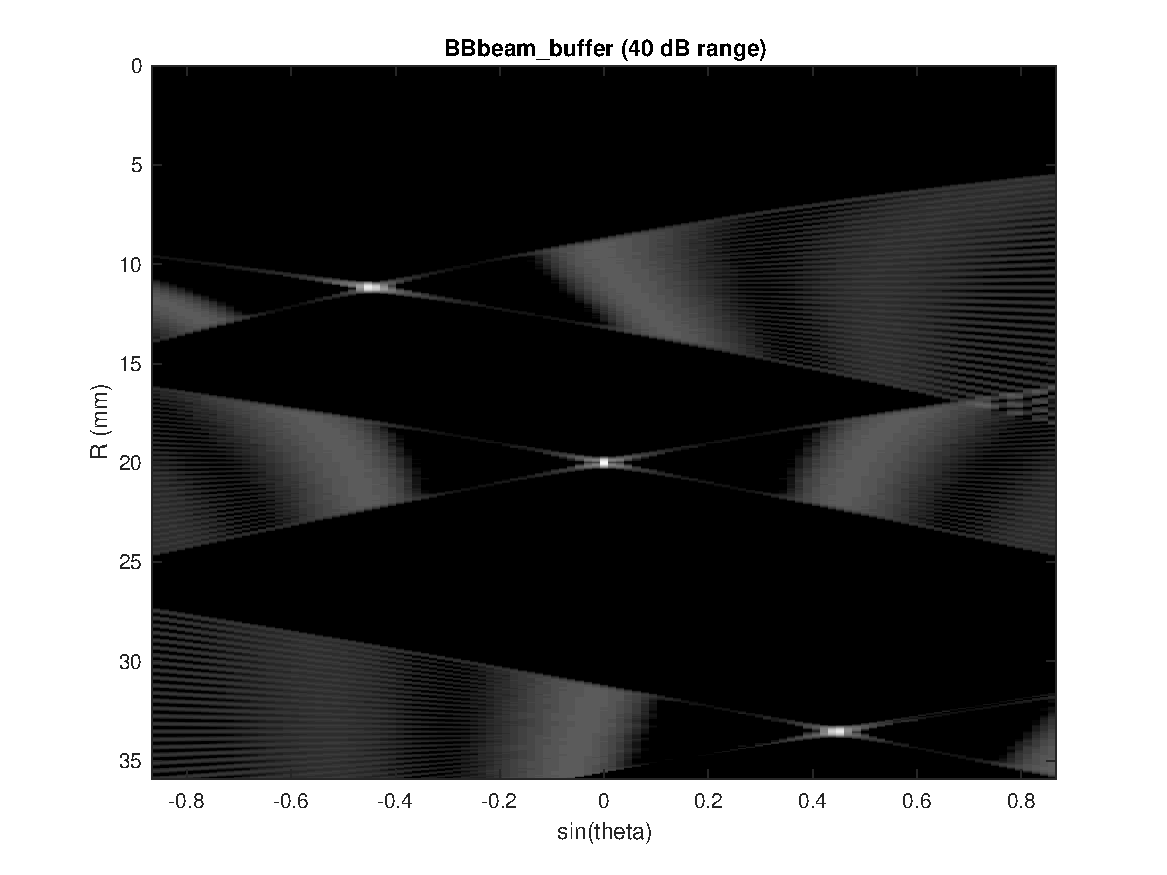
\includegraphics[width=0.6\textwidth]{src/RF/b-8-everyones.pdf}
    \caption{(f) Beam buffer of RF (40 dB dynamic range)}
    \label{fig:RF-everyones-40db}
\end{figure}
In Figure \ref{fig:RF-everyones-40db}, the contrast between area around focus point and the other is much worse than 
Figure \ref{fig:RF-b-40db}. This is because we only use data recieved from half number of elements and the energy difference
of focus point area and the others will get much smaller. So the contrast becomes worse.

\subsection{Sector Images}
Figure \ref{fig:RF-ones-sector} and \ref{fig:Base-ones-sector} show the sector images in (c), respectively.
\begin{figure}[H]
    \centering
    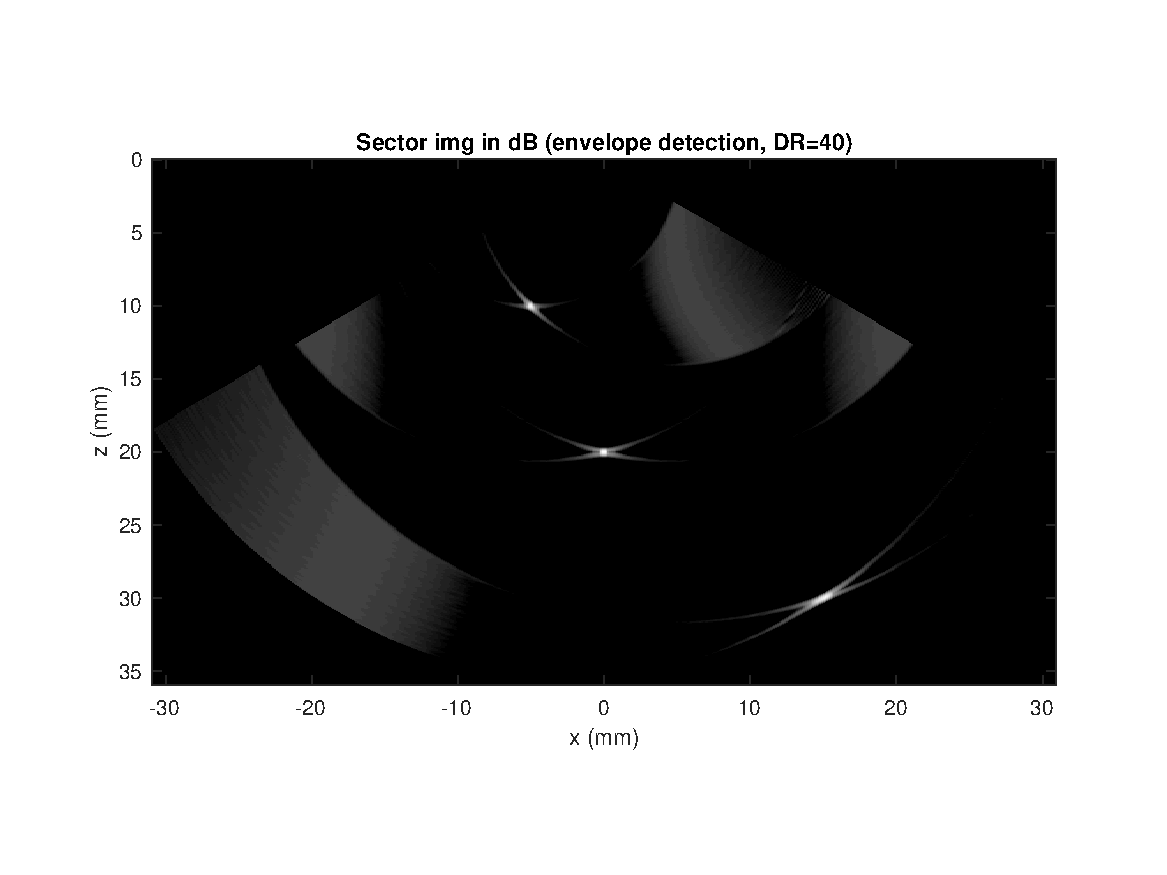
\includegraphics[width=0.6\textwidth]{src/RF/b-9-ones.pdf}
    \caption{(c) Sector image of RF (40 dB dynamic range)}
    \label{fig:RF-ones-sector}
\end{figure}
\begin{figure}[H]
    \centering
    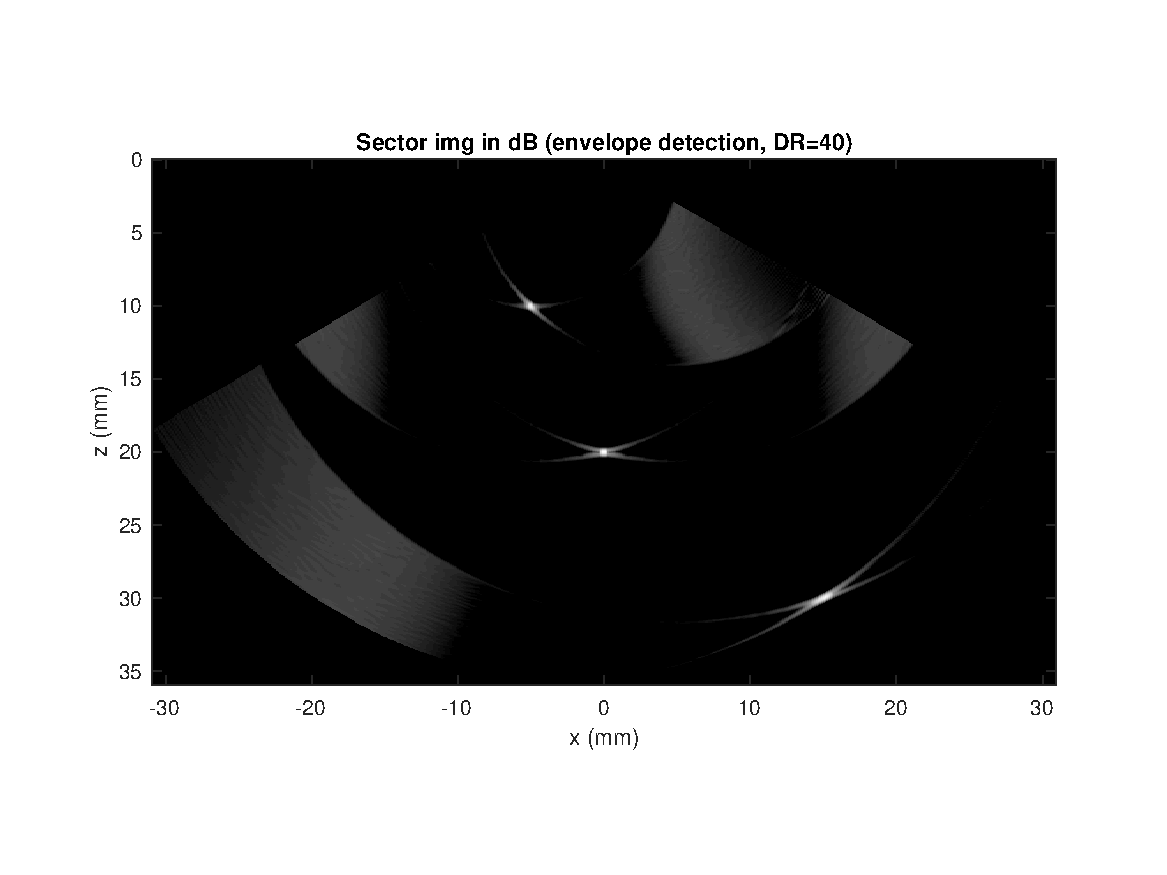
\includegraphics[width=0.6\textwidth]{src/Base/b-6-ones.pdf}
    \caption{(c) Sector image of Baseband (40 dB dynamic range)}
    \label{fig:Base-ones-sector}
\end{figure}

Figure \ref{fig:RF-hanning-sector} show the result of (d).
\begin{figure}[H]
    \centering
    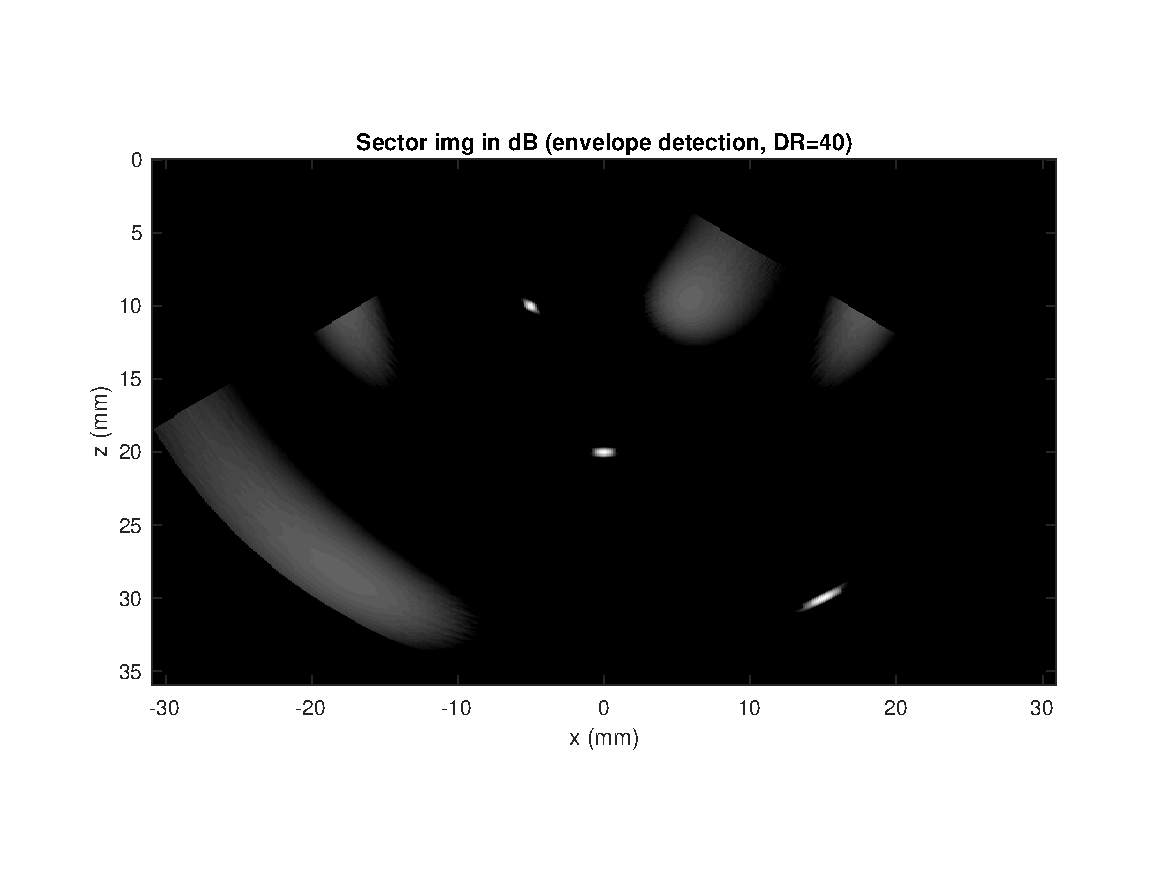
\includegraphics[width=0.6\textwidth]{src/RF/b-9-hanning.pdf}
    \caption{(d) Sector image of RF (40 dB dynamic range)}
    \label{fig:RF-hanning-sector}
\end{figure}

Figure \ref{fig:RF-2pitch-sector} show the result of (e).
\begin{figure}[H]
    \centering
    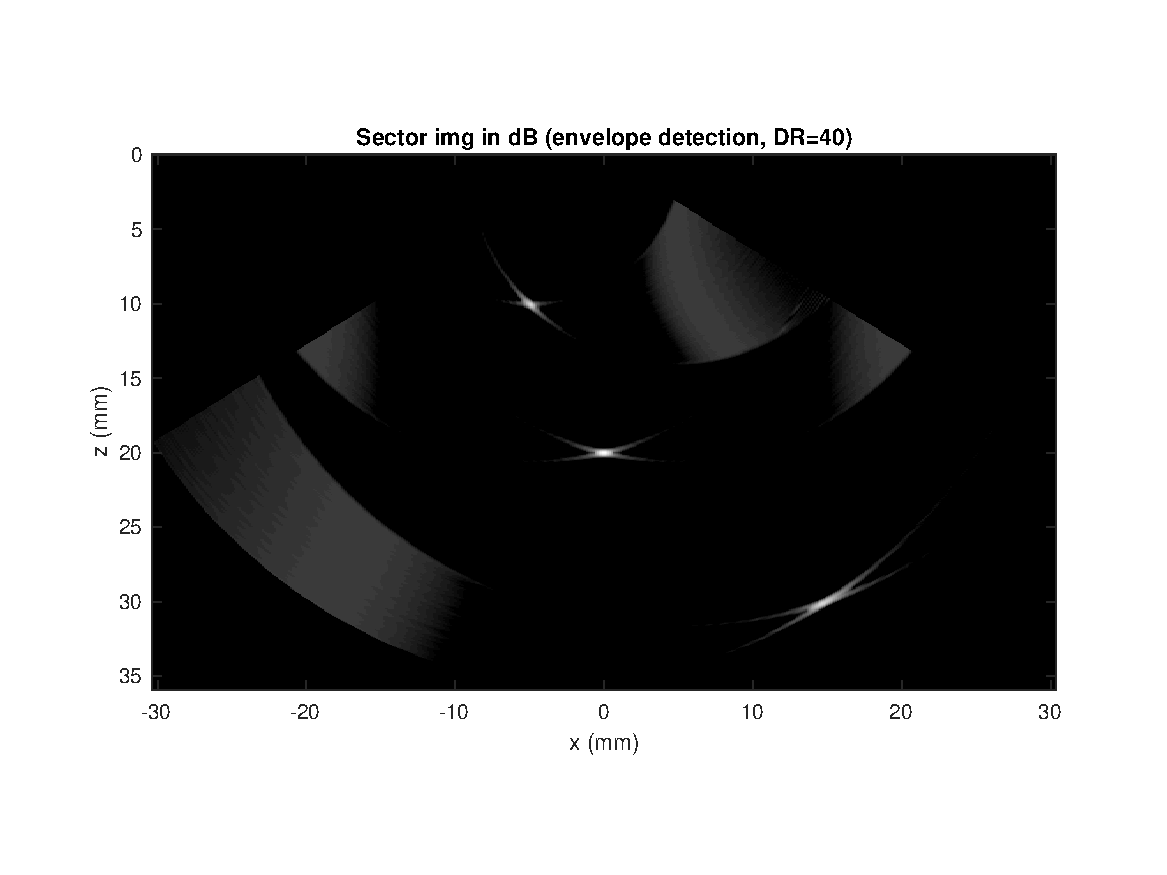
\includegraphics[width=0.6\textwidth]{src/RF/b-9-2pitch.pdf}
    \caption{(e) Sector image of RF (40 dB dynamic range)}
    \label{fig:RF-2pitch-sector}
\end{figure}

Figure \ref{fig:RF-everyones-sector} show the result of (f).
\begin{figure}[H]
    \centering
    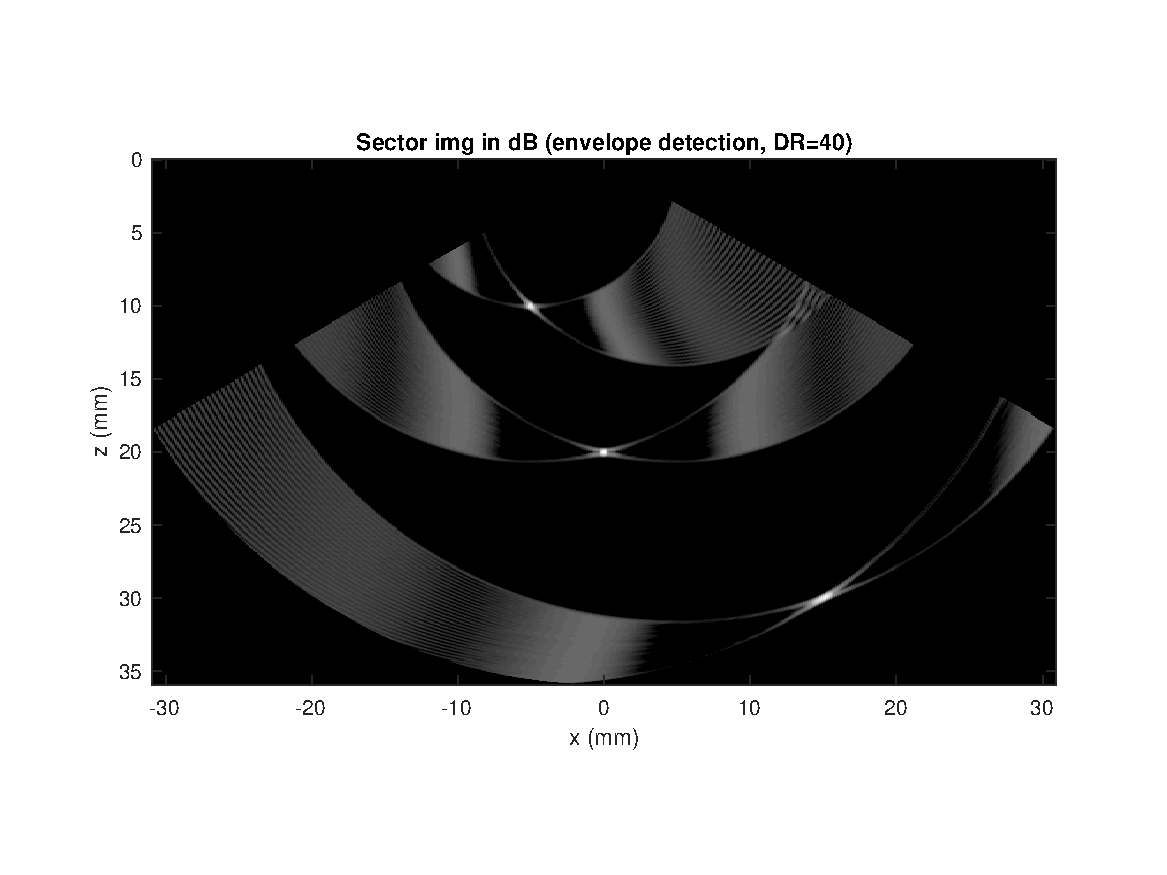
\includegraphics[width=0.6\textwidth]{src/RF/b-9-everyones.pdf}
    \caption{(f) Sector image of RF (40 dB dynamic range)}
    \label{fig:RF-everyones-sector}
\end{figure}

\end{document}        
   














